\documentclass[10pt,a4paper]{article}
\usepackage[utf8]{inputenc}
\usepackage{amsmath}
\usepackage{amsfonts}
\usepackage{amssymb}
\usepackage{a4wide} %Wider margins
\usepackage[english]{babel} %English dictionary for hyphenation and definitions, e.g. Table vs. Tabel
\usepackage[official]{eurosym} %Support for Euro-sign
\usepackage[utf8]{inputenc} %Support for internationalization, e.g. é vs.\’e
\usepackage{amsmath,amssymb,amsthm} %Support for mathematical formulas and symbols
\usepackage{fancyhdr} %Fancy headers
\usepackage{hyperref} %Creates clickable links
\usepackage{graphicx} %Support for grahpics
\usepackage{nopageno} %Support for removal of pagenumbers
\usepackage{tabularx}
\usepackage{enumitem}
\usepackage{xspace}
\usepackage{algorithm,algpseudocode}
\usepackage{float}
\usepackage{mathtools}
\usepackage[dvipsnames]{xcolor}
\usepackage[titletoc,toc,title]{appendix}
\usepackage{listings}
\graphicspath{ {./ThesisFigures/} }

\hypersetup{
    pdftitle={}, %PDF-file will be given a proper title when viewed in a reader
    hidelinks %PDF-file will be given clickable, yet not visible links when viewed in a reader
}
\newcommand{\documenttitle}{Biomedical Data Analysis }
\newcommand{\documentsubtitle}{Discovering and reviewing several analysis techniques}


\newcommand{\true}{{\sc True}\xspace}
\begin{document}
	
	\begin{titlepage}
		
		\center
		
		\vspace*{3cm}
		
		\textbf{\huge \documenttitle}
		
		\textit{\LARGE \documentsubtitle}
		
		\vspace*{2cm}
		
		\large
		\centering
		T.P.A.~\textsc{Beishuizen}~(0791613)\\
		Biomedical Engineering - Computational Biology\\
		Data Engineering - Information Systems\\
		Eindhoven, University of Technology\\
		Email: \texttt{t.p.a.beishuizen@student.tue.nl}
		
		\vfill
		
		\vspace*{1cm}
		
		\today
		
	\end{titlepage}
	
	\tableofcontents
	
	%\newpage
	
	\pagestyle{fancy}
	%Abbreviations used by fancyhdr:
	%E Even page
	%O Odd page
	%L Left field
	%C Center field
	%R Right field
	%H Header
	%F Footer
	\fancyhead{} % clear all header fields
	\fancyfoot{} % clear all footer fields
	\renewcommand{\headrulewidth}{0.4pt}
	\renewcommand{\footrulewidth}{0.4pt}
	
	\fancyhead[L]{\rightmark}
	\fancyfoot[C]{\thepage}
	\fancyhead[R]{T.P.A. Beishuizen}
	
	
	\clearpage
	
	\section{Introduction}
	
	% Quick explanation for graduation project
	At the Computational Biology department (cBio) of Biomedical Engineering (BME), many requests are made to analyse gathered data. This data usually stems from research in hospitals, but also data from other research groups and publicly known data. With the vast number of data sets that are available, a framework on data analysis would be valuable. This framework would improve efficiency of this data analysis, as it would help choosing the best analysis approaches. 
	
	% Explanation for this document
	Before this framework is made however, first extensive research must be done on the already available analysis techniques. Many different approaches are used by researchers. These should be searched for and compared with each other, first using literature and second by actual use. This document focuses mainly on the literature part and explores the different techniques by analysing the articles.
	
	% Document lay-out
	At first the focus will mainly be on statistical methods. Different 
	techniques will be explained as well as the programs that can be used for 
	these statistical techniques. The second topic will be about machine 
	learning, and more specifically deep learning. 
	
	\clearpage
	
	\section{Statistical Analysis}
	
	% Quick summary of statistical analysis
	Statistical analysis consists of statements derived from large data sets that are often visualized in tables, graphs and charts. These statements are made on the basis of hypotheses and the analyses that either back up or reject those. The available data sets need to have a reasonably sized population so the statistical hypotheses can be tested. \cite{woolson2011statistical} 
	
	% When to use statistical analysis? -- Find a reference for this
	The statistical approach is mainly used for drawing conclusions on the 
	data. When focusing on summarizing the data, inductive conclusions can be 
	made which then can be used in the biomedical world. Techniques that are 
	specifically useful for biomedical data are all combined in the term 
	biostatistics. \cite{woolson2011statistical} 
	
	% The way data should look like
	To be able to use statistical analysis, the data should be quantitative. The data should be a population of data points and usually the size influences the accuracy of the outcome. Since most biomedical data stems from experiments on patients, the data usually is quantitative and can be analysed by statistical techniques. \cite{sapsford2006data}
	
	% Chapter layout
	In this statistical analysis chapter, first some concepts are discussed. 
	Since for every data set the to be used computations are different, only 
	the basic ones are used to keep the report from irrelevant explanations. 
	Afterwards, five different programs or frameworks are discussed for their 
	approach to statistical analyses. Afterwards these five are compared by 
	literature and by personal testing.
	
	\clearpage
	
	\subsection{Statistical Research Topics}
	
	% Introduction statistical research
	Statistical research on its own has many applications. A selection of those 
	that are relevant for Biomedical data are discussed in here. Important in 
	statistical analysis is the presence of hypotheses. When doing this 
	analysis, the researcher has an expectation of the outcome. An example of 
	this would be having a data set of people of age and number of 
	grandchildren. The hypothesis could be: \textit{$H_0$: There is a 
	correlation between people's age and the number of grandchildren.} Then at 
	the end this or an alternate hypothesis $H_1$ can be either validated or 
	rejected.\cite{heiberger2004statistical}
	
	\subsubsection{Descriptive Statistics}
	
	% Introduction of descriptive statistics
	Descriptive statistics is a collection of methods for data analysis based around its variables. Data set variables are either nominal (categorical or grouped), ordinal (Ranked relatively) or continuous (Ranked with equal intervals). Descriptive statistics takes these variables and computes details of their distribution (Table \ref{tab:DescrStatEx}). \cite{FISHER200993} These then summarize the data for the scientist analysing it. The newly created summary can be used for further statistical research, for example by comparing different populations or variables. \cite{woolson2011statistical}
	
	\begin{table}[h!]
		\centering
		\caption{Descriptive Statistics examples\cite{FISHER200993}}
		\label{tab:DescrStatEx}
		\begin{tabular}{|l|l|l|l}
			\cline{1-3}
		\textbf{\begin{tabular}[c]{@{}l@{}}Variable \\ distribution\end{tabular}} & \textbf{\begin{tabular}[c]{@{}l@{}}Analysis terms \\ Center oriented\end{tabular}} & \textbf{\begin{tabular}[c]{@{}l@{}}Analysis terms\\ Spreading oriented\end{tabular}}                            &  \\ \cline{1-3}
			Nominal                                                                                           & Mode                                                                                                       & Frequency distribution                                                                                                                  &  \\ \cline{1-3}
			Ordinal                                                                                           & \begin{tabular}[c]{@{}l@{}}Median \\ Mode\end{tabular}                                                     & \begin{tabular}[c]{@{}l@{}}Frequency distribution\\ Percentiles\\ Minimum/Maximum\\ Range\end{tabular}                                  &  \\ \cline{1-3}
			Continuous                                                                                        & \begin{tabular}[c]{@{}l@{}}Mean\\ Median\\ Mode\end{tabular}                                               & \begin{tabular}[c]{@{}l@{}}Frequency distribution\\ Percentiles\\ Quartiles\\ Minimum/Maximum\\ Range\\ Standard Deviation\end{tabular} &  \\ \cline{1-3}
		\end{tabular}
	\end{table}

	% Visualization of descriptive statistics
	Aside from the aforementioned summary of the variables, descriptive statistics also consists of methods to properly visualize those. For nominal and ordinal data, histograms (Figure \ref{fig:HistEx}) and bar charts are often use to show in a easily understandable way how they are distributed. For continuous data box plots (Figure \ref{fig:BoxEx}) can be used as well to show specific details of the distribution. \cite{dupont2009statistical}
	
	\begin{figure}[h!]
		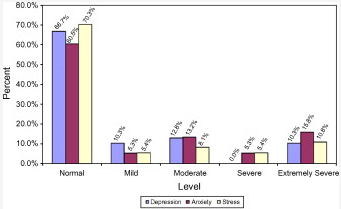
\includegraphics{HistogramExample.PNG}
		\caption{An example of a histogram of ordinal data. The depression, anxiety and stress scale of women with an acute coronary syndrome is shown. the data shows that over sixty percent rates themselves as normal. \cite{FISHER200993}}
		\label{fig:HistEx}
	\end{figure}

	\begin{figure}[h!]
	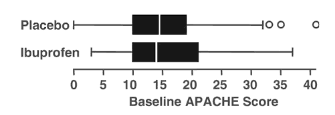
\includegraphics{BoxplotExample.PNG}
	\caption{An example of a box plot of continuous data. The distribution of the APACHE score (Acute Physiology And Chronic Health Evaluation) was given for users of ibuprofen and placebo. The box plot doe snot only show the minimum, maximum and mean, but also quartiles and possible outliers. \cite{dupont2009statistical}}
	\label{fig:BoxEx}
	\end{figure}
	
	\subsubsection{Probability Concepts}
	
	% Introduction
	When using biomedical data, it usually contains some phenomena that seem random and affect data values. Modelling and analysis of those data phenomena is hard, due to his unpredictability. A probabilistic approach can be used to tackle this. \cite{shiavi2010introduction}
	
	% Probability meaning
	Values that seems to have a random part can be measured multiple times. 
	When looking at multiple measurements an average can be found within their 
	distribution in the sample space. The probability of a value to be within a 
	certain interval is always a number between 0 and 1. The probability of a 
	value to be in the sample space is 1, as it the complete interval. 
	\cite{shiavi2010introduction}
	
	% Probability Distribitions
	Another aspect of probability is about the several distributions. These 
	show the total probability for a value to be on a certain interval. There 
	are two different kinds of probability distributions: discrete and 
	continuous. The difference between these two is the spacing between the 
	possible values. Values from continuous distributions can take every value, 
	whereas values from discrete distributions are limited and the possible 
	values have spacings between them.\cite{heiberger2004statistical}
	
	% Binomial distribution
	Binomial distribution is the most common example of a discrete distribution 
	(Figure \ref{fig:BinomDistEx}). This distribution can be seen as a number 
	of $n$ independent trials that have a success rate of $p$, with $p$ being a 
	number on the interval $(0,1)$. This distribution has a mean of $\mu = np$ 
	and standard deviation of $\sigma = \sqrt{np(1-p)}$. 
	\cite{heiberger2004statistical}
	
	\begin{figure}[h!]
		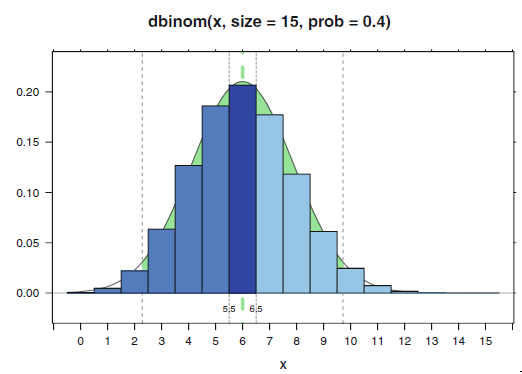
\includegraphics[scale=0.5]{BinomDistExample.PNG}
		\caption{An example of a binomial distribution, a discrete probability 
		distribution. In this example there were $n =  15$ trials with a 
		success rate of $p = 0.4$. \cite{heiberger2004statistical}}
		\label{fig:BinomDistEx}
	\end{figure}

	% Normal distribution
	The most common continuous probability distribution is called a normal 
	distribution (Figure \ref{fig:NormDistEx}). This distribution is bell 
	shaped and symmetric around the mean $\mu$, with a standard deviation 
	$\sigma$. The standard normal distribution $Z$ has a $\mu = 0$ and $\sigma 
	= 1$ and can be made with a modification on a regular normal distribution 
	$X$: $Z = \frac{X-\mu}{\sigma}$. \cite{heiberger2004statistical}

	\begin{figure}[h!]
		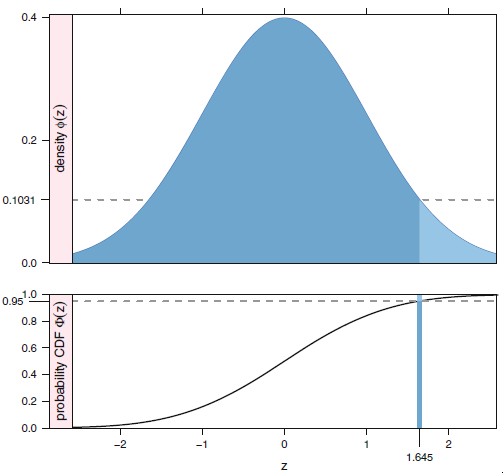
\includegraphics[scale=0.5]{NormDistExample.PNG}
		\caption{An example of a normal distribution, a continuous probability 
		distribution. This example is the standard normal distribution with 
		mean $\mu =  0$ and standard deviation $\sigma = 1$. 
		\cite{heiberger2004statistical}}
		\label{fig:NormDistEx}
	\end{figure}
	
	% Student's T distribution
	The third distribution that will be discussed is the student's 
	t-distribution, another continuous distribution (Figure 
	\ref{fig:StudTDistEx}). This one is very similar 
	to the normal distribution discussed earlier. The student's t distribution 
	has a sample size of $n$ and a sample standard deviation of $s$. The 
	standard distribution can be found with the formula $Z = \frac{X-\mu}{s / 
	\sqrt{n}}$ The larger the sample size $n$, the closer $s$ will get to 
	$\sigma$ of a normal distribution, so an infinite sample size $n$ is a 
	normal distribution.\cite{heiberger2004statistical}
	
	\begin{figure}[h!]
		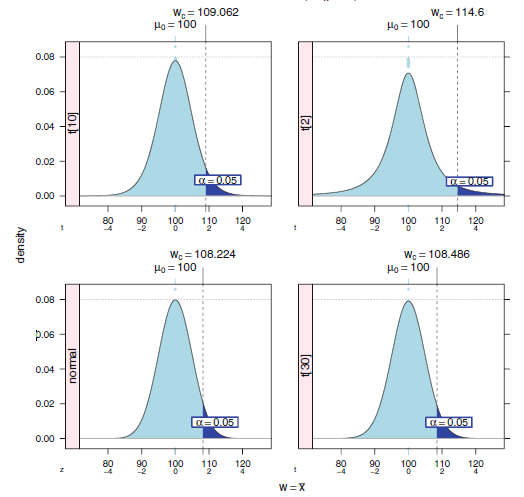
\includegraphics[scale=0.5]{StudTDistExample.PNG}
		\caption{An example of a 3 student's t distributions and a normal 
		distribution. With an sample size $n$ becoming higher, the standard 
		deviation $s$ comes closer to normal distribution standard deviation 
		$\sigma$. \cite{heiberger2004statistical}}
		\label{fig:StudTDistEx}
	\end{figure}
	
	% Famous tests that find out the goodness of fit
	Several tests are used to find out if a data set can be fits a certain 
	distribution. The "Goodness of fit" is then tested. The Chi-Square and 
	Kolmogorov Smirnov are such tests. There may be more powerful and 
	specialized ones though, for example the Shapiro Wilk for normality 
	testing. \cite{heiberger2004statistical}
	
	\subsubsection{Interval testing}
	
	%Introduction
	On the previously discussed probability distributions specific intervals 
	can be computed. A confidence interval can show the interval where a 
	certain value should be in. This can be done for an unknown mean of a 
	distribution or an unknown population proportion in a t distribution. These 
	intervals are made similar to this one, the confidence interval of the 
	mean, with 
	mean $\hat{y}$, confidence number $z$, percentage cut-off $\alpha$, 
	standard deviation $\sigma$ and 
	population sample $n$ (Equation \ref{eq:CI}).\cite{heiberger2004statistical}
	
	\begin{equation}
		\label{eq:CI}
		(\hat{y} - z_{\frac{\alpha}{2}}\frac{\sigma}{\sqrt{n}}, \hat{y} + 
		z_{\frac{\alpha}{2}}\frac{\sigma}{\sqrt{n}})
	\end{equation}	
	
	\subsubsection{Group comparisons}
	
	% Introduction
	The previously discussed confidence intervals can be used to find out 
	whether two data sets are similar in terms of mean and variance. If the 
	confidence intervals of the means of both data sets then the two data sets 
	could be describing the same distribution. Its independence can then be 
	proven by comparing their confidence intervals. 
	\cite{heiberger2004statistical}
	
	% Explanation comparison mean
	The independence has two different parts. Two data sets can be independent 
	comparing their means and they can be independent comparing their 
	variances. The more important one of the two is when means are compared, as 
	then they can be substantially different. To test whether two data sets are 
	independent on their mean, a series of tests can be done ( 
	\ref{tab:IndepTest}). For these tests it makes a difference whether the 
	unknown variance is common, different or the data is 
	paired.\cite{heiberger2004statistical}
	
	\begin{table}[h!]
	\centering
	\caption{Formulas to compute whether two samples are independent by means. 
	The parameters $s_{\Delta\bar{y}}$ and $t_{calc}$ can be three different 
	values (Table \ref{tab:sdyandtcalc})\cite{heiberger2004statistical}. The values for the mean $\mu$, }
	\label{tab:IndepTest}
	\begin{tabular}{llllll}
		\hline
		 &  & 
		\multicolumn{2}{l}{\textbf{Tests}} & 
		\textbf{Confidence Interval} & \textbf{}               \\ \cline{3-6} 
		\textbf{H0}              & \textbf{H1}              & \textbf{Rejection 
		region}   & $p$-value                      & 
		\textbf{Lower}               & \textbf{Upper}          \\ \hline
		$\mu_1 \leq \mu_2$                  & $\mu_1 > \mu_2$       & 
		$t_{calc} 
		> t_\alpha$       & $P(t > t_{calc})$      & 
		$((\bar{y}_1 
		- \bar{y}_2) - t_\alpha s_{\Delta \bar{y}}$,       & 
		$\infty)$                     \\
		$\mu_1 \geq \mu_2$                  & $\mu_1 < \mu_2$          & 
		$t_{calc} 
		< -t_\alpha$          & $P(t < t_{calc})$         & 
		$(-\infty$,                        & $(\bar{y}_1 - \bar{y}_2) + 
		t_\alpha 
		s_{\Delta \bar{y}})$ \\
		$\mu_1 = \mu_2$                  & $\mu_1 \neq \mu_2$                  
		& 
		$|t_{calc}| > t_{\frac{\alpha}{2}}$     & $P(t >
		|t_{calc}|)$  & $((\bar{y}_1 - \bar{y}_2) - 
		t_{\frac{\alpha}{2}} 
		s_{\Delta\bar{y}}$ 
		,     & $(\bar{y}_1 - \bar{y}_2) + t_{\frac{\alpha}{2}} 
		s_{\Delta 
		\bar{y}})$  
		\\ 
		\hline
	\end{tabular}
	\end{table}
	
	\begin{table}[h!]
		\centering
		\caption{The values of $s_{\Delta\bar{y}}$ and $t_{calc}$ for data sets 
		with common unknown variance, uncommon unknown variance and paired 
		data. \cite{heiberger2004statistical}}
		\label{tab:sdyandtcalc}
		\begin{tabular}{lll}
			\hline
			\textbf{Data set}  & \textbf{$s_{\Delta\bar{y}}$}     & 
			\textbf{$t_{calc}$}                                                
			              \\ \hline
			Common variance    & $s_{\Delta\bar{y}} = s_p \sqrt{\frac{1}{n_1} + 
				\frac{1}{n_2}}$ & 
			$t_{calc} = \frac{\bar{y}_1-\bar{y}_2}{s_p \sqrt{\frac{1}{n_1} + 
			\frac{1}{n_2}}}         $                                      \\
			Different variance & $s_{\Delta\bar{y}} = s_{\bar{y}_1 - 
			\bar{y}_2}$    & 
			$s_{(\bar{y}_1-\bar{y}_2)} =\sqrt{\frac{s^2_1}{n_1} + 
			\frac{s^2_2}{n_2}}$, and $t_{calc} = \frac{\bar{y}_1 - 
			\bar{y}_2}{s_{(\bar{y}_1-\bar{y}_2)}}$ \\
			Paired data        & $s_{\Delta\bar{y}} = \bar{s}_d$           & 
			$s_{\bar{d}} = s_d / \sqrt{n}$, and $t_{calc} 	
			=\frac{\bar{d}}{s_{\bar{d}}}$                                       
			  
			 
			     \\
			 \hline
		\end{tabular}
	\end{table}
	
	% Explanation comparison variance
	To find out whether variances of two data sets could be common, a new value 
	$F$ is introduced with the formula $F = \frac{s_1^2}{s_2^2}$. Since this $F 
	= 1$ is the most ideal situation (both variances being equal), an equation 
	can be made in which the boundaries can be specified (Equation 
	\ref{eq:FVarInt}). In this equation $F_{low} = F_{1-\frac{\alpha}{2},n_1-1, 
	n_2-1}$ and $F_{high} =  F_{1-\frac{\alpha}{2},n_2-1, n_1-1}$, the upper 
	percentage points with the $n_1 - 1$ and $n_2 - 1$ or $n_2 -1$ and $n_1 - 
	1$ degrees of freedom respectively. 
	\cite{heiberger2004statistical}
	
	\begin{equation}
		\label{eq:FVarInt}
		(\frac{s_1^2}{s_2^2}\frac{1}{F_{low}}, \frac{s_1^2}{s_2^2}F_{high})
	\end{equation}
	
	% Tests for data
	If data is paired (Table \ref{tab:IndepTest}), to test if their means are 
	paired is usually done with a t-test. A similar version, the two sample 
	t-test, is the way to go when the distribution is known of the data set. A 
	specific way to tests multiple groups at the same time is the one-way 
	analysis of variance (ANOVA). This t-test is preferred over other test due 
	to his power compared to the other tests. \cite{heiberger2004statistical}
	
	% Tests for non-parametric (paired) data
	Data can also not follow any specific distribution. In those cases 
	Non-parametric statistical procedures will be used. An example would be the 
	Sign test, when a certain median is taken and found out if there are enough 
	data points above and under that median. This Sign test can also be used 
	with paired populations and find out whether there is a significant number 
	of data points from one of the sets lower than the data points from the 
	other set. An upgraded version of this Sign test is called Wilcoxon 
	Signed-Ranks Test, which also takes the magnitude of the data into 
	account.\cite{heiberger2004statistical}
	
	% Tests for non-parametric unpaired data
	If the data is not paired, the Mann-Whitney Test may be a good choice. This	
	test is related to the two sample t-test, however uses medians instead of 
	means. The more than two sample testing version of the Mann-Whitney Test is 
	the Kruskal-Wallis test. This test should be used if some of the 
	populations do not seem to be uniformly distributed enough for an ANOVA 
	test.\cite{heiberger2004statistical}
	
	\clearpage
	
	\subsection{Statistical Programs}
	
	\subsubsection{SAS}
	
	% SAS explanation
	Statistical Analysis System (SAS) is a system used for statistical 
	analysis. It can be used to perform a big variety of those with ease. 
	Scientist can learn SAS quickly to perform small statistical computations 
	for quick results. Within SAS a variety of algorithms are available for 
	analysis. This simplicity of calling those algorithms makes SAS very time 
	efficient. \cite{o2013step}
	
	\subsubsection{SPSS}
	
	% SPSS explanation
	SPSS is the statistical program with the most diverse users. SPSS is very 
	user-friendly and easy to use when not familiar in either programming or 
	when the there is only need for basic statistical analysis. Due to these 
	advantages in educational research SPSS is widely used, especially by the 
	social studies in need of these analysis techniques. \cite{muijs2010doing}
	
	\subsubsection{R}
	
	% R explanation
	R is one of the more well known statistical computing language for people who have experience in programming. It provides a language as well as statistical procedures to use for their analysis. Both SAS and SPSS created extensions for R, so it can be used in theirs as well. This is less intuitive, due those two being very similar. \cite{muenchen2011r}
	
	\subsubsection{Python}
	
	% Python explanation
	Python is widely known for being an open source programming language with a 
	relatively low bar to learn it. It was not often used for scientific 
	analyses. Due to the maturity of several useful library as Numpy and Scipy 
	however, python's market share is growing. Its open source element 
	increases the usability over time as well. At last, since python is also 
	used for other projects not involving statistics, scientists may already 
	know the language. 
	\cite{mckinney2010data}
	
	\subsubsection{MATLAB}
	
	% Matlab explanation
	Matlab is not necessarily known for its statistical analysis, but more for 
	its good way of handling biomedical data. Biomedical scientists and 
	engineers are often familiar with MATLAB and its clear way of writing 
	commands to analyse data. For statistical analysis extensions are 
	available, an example would be the computational statistics toolbox. Also 
	on the internet, many freely available user-created functions can be found, 
	which can be used to the scientist's advantage.
	\cite{martinez2007computational}
	
	\subsubsection{Comparisons programs}
	
	% First example comparisons
	Many comparisons are made for scientists which statistical program is best 
	to use. A good scheme was made by Jeroen Kromme, a data scientist of 
	Cmotions that is involved with bringing data analysis to other scientists 
	(Figure \ref{fig:StatProgComp}). He compares the fairly accessible programs 
	SAS and SPSS with the more potential programs R and 
	Python.\cite{BlogKromme2017}
	
	\begin{figure}[h!]
		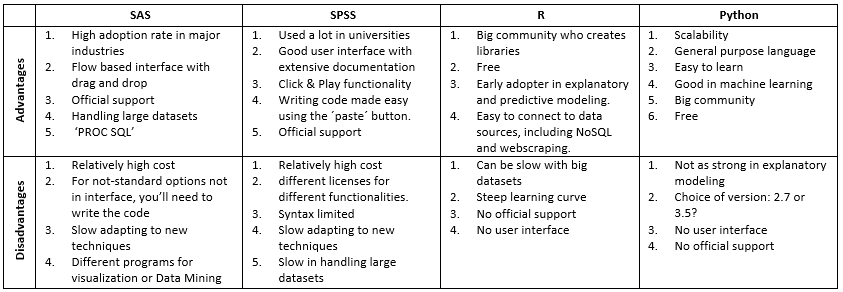
\includegraphics[width=\textwidth]{StatProgComp.PNG}
		\caption{Advantages and Disadvantages of the statistical programs SAS, 
		SPSS, R and Python.\cite{BlogKromme2017}}
		\label{fig:StatProgComp}
	\end{figure}
	
	 % Second example comparisons
	 Another article has been written by Kunal Jain that compares the 
	 commercially used SAS with the academic R and the high potential Python. 
	 He rates the programs on different aspects with what he shows that Python 
	 has the best potential of the three (Figure 
	 \ref{fig:StatProgGrades}).\cite{BlogJain2017}
	
	\begin{figure}[h!]
		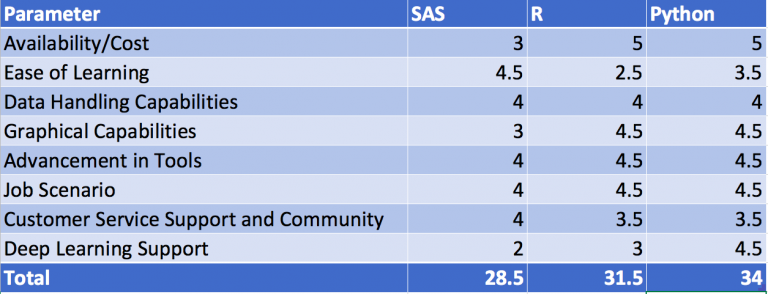
\includegraphics[width=\textwidth]{StatProgGrades.PNG}
		\caption{Grades for SAS, R and Python on different aspects of using a 
		program for statistical analysis.\cite{BlogJain2017}}
		\label{fig:StatProgGrades}
	\end{figure}
	
	% Combinatons of programs
	Combinations of the statistical programs is also possible. SAS and SPSS are 
	very similar to each other and switching between those is 
	not hard to do. Both of these use extensions that allows the user to work 
	with R functions. This is useful as R has more variety in their functions 
	compared with SAS and SPSS.
	\cite{muenchen2011r}
	
	% Final comparisons
	These explained surveys and more \cite{BlogWillems2014} 
	\cite{BlogSupport2017} show that these programs all have a different 
	approach. SPSS is used by the scientists and companies that don't need very 
	advanced techniques. SAS extends the the usability of SPSS by a little and 
	is provided by support, therefore companies that need a bit more advanced 
	statistical analyses prefer to use SAS. R is a widely known useful program 
	that is mainly used in the academic world by scientists that know a bit of 
	programming and need more in-depth analyses. Python is not widely used, yet 
	but is on the rise due to its popularity for other programming sciences, as 
	well.
	
	\subsubsection{Personal comparisons}
	
	% Testing of statistical programs
	All of these statistical programs have been tested personally, too. This 
	was done in past projects for courses at the TU/e The 
	final comparisons of the articles match the outcome of those findings. 
	
	% Matlab, SPSS and SAS
	SPSS and SAS can do numerous things statistically, however it is still very 
	basic compared to R and Python. Since biomedical engineers are known to 
	process their data in MATLAB and python, it is not worth it to pre-process 
	data to use in SAS and SPSS when MATLAB and python can do about the same 
	things. If the only need is fairly simple statistical computations, MATLAB 
	will be sufficient for that. If the there is need for more complex 
	computations, SAS and SPSS most likely would not be able to do those easily 
	anyways. 
	
	% R and python
	If more complex statistical analyses are needed, it would be smarter to 
	look at R and python for use. They both work on a similar level and both 
	have an advantage over the other. If a scientist is not familiar with 
	complex statistical analyses or with either language, R might be better for 
	him. R is more widely used and therefore more material is available for 
	help. Scientists that do know python or are already working with it, are 
	better of doing the statistical analyses with python. There is no need 
	learning a new language when it would only take up more time.
	
	\clearpage
	
	\section{Deep Learning}
	
	% Introduction to Deep Learning
	As computers are becoming smarter and smarter, the idea of computers 
	learning how to tackle various problems is bigger than before. Also the 
	size of data sets is growing two, which makes current ways of extracting 
	information harder to use. The idea of 
	giving computers a way to learn from experience and teach them how to cope 
	with examples for treating real data the right way is called deep learning. 
	\cite{Goodfellow-et-al-2016} Deep learning is structurally used more in the 
	biomedical environment to explain several concepts, especially considering 
	images and the usage of neural networks.\cite{greenspan2016guest}
	
	% Talking about Deep Learning topics
	The whole idea of a computer gaining experience from finding patterns in 
	the data is called machine learning. Deep learning is a sub section of 
	machine learning as deep learning tries to solve problems by combining 
	multiple small solutions. These small solutions are then connected in a 
	network, that is often called a artificial neural network (ANN), resembling 
	the neural network in a human brain.\cite{Goodfellow-et-al-2016}
	
	\clearpage
	
	\subsection{Basic Machine Learning}
	\label{subsec:MachineLearning}
	
	% Introduction
	As deep learning is a specific kind of machine learning, knowing the 
	important basics of machine learning is necessary. This is divided in three 
	different parts, the task, performance measurement and the experience 
	gained.\cite{Goodfellow-et-al-2016}
	
	\subsubsection{Tasks}
	
	% Task description
	The task of a machine learning program is to solve problems that can not be 
	solved by humans only. This way of solving requires a different mindset in 
	programming. The program must be made so it knows how to solve a problem 
	instead of manually telling the program how to solve it. Tackling a problem 
	in the case of machine learning usually is done by having it process 
	examples that are a collection of features. The example is a data point 
	which details are described by those features. What needs to be done with 
	those examples can be different.\cite{Goodfellow-et-al-2016}
	
	% Classification
	One task the program could do is specify a specific label from a number of 
	categories. The examples all should be divided between several groups and 
	machine learning tries to find the correct group for every example. This 
	can be done multiple ways. Examples are in a discrete way (every example 
	has one group) or in a probabilistic way (every example has a certain 
	chance to be part of some groups).\cite{Goodfellow-et-al-2016}
	
	% Regression
	Another task the program could do is predict a numerical value for the 
	examples. This is similar to classification only the answer is not limited 
	to a number of categories. Instead it can be any value on a numerical 
	interval. \cite{Goodfellow-et-al-2016}
	
	% Other tasks
	Classification and regression are the most commonly used tasks within 
	machine learning. Other less used tasks could be to translate data to a 
	structured representation, to detect errors in the examples or remove noise 
	from the data. All off these tasks could be tackled using machine 
	learning.\cite{Goodfellow-et-al-2016}
	
	\subsubsection{Performance Measurement}
	
	%Introduction performance measurement
	When using machine learning, the performance of the algorithm is important. 
	The program should not only use the data to create output, but this output 
	must be correct as well. To measure this correctness, the accuracy is often 
	measured. This accuracy is the percentage of examples that give the correct 
	output. An error rate can be used as a performance measurement too, the 
	number of examples that give an incorrect 
	output.\cite{Goodfellow-et-al-2016}
	
	% Using a test set
	Data is used when training a machine learning algorithm. The algorithm is 
	made to be as effective as possible for this training data, therefore the 
	accuracy is supposed to be high for that data. This training data is 
	usually just a subset of all possible data though and therefore the actual 
	accuracy may be lower. To find this out, a separate test set can be made 
	alongside the training set. This test set is then only used to find this 
	accuracy.\cite{Goodfellow-et-al-2016}
	
	% Further perfomance discussion
	The performance measurements also require further thoughts than the 
	accuracy and test sets. It may very well be that some categories in 
	classifications are more important to be right (e.g. high risk patients) or 
	the penalty for big deviations in regression may be bigger than needed. 
	These things all need to be considered before measuring the accuracy. 
	\cite{Goodfellow-et-al-2016}
	
	\subsubsection{Experience}
	
	% Introduction Experience
	There are superficially spoken two kinds of machine learning, unsupervised 
	or supervised. The difference between those is the experience they are 
	allowed to have during its training. This training is done with a specific 
	idea in mind that differs for these two 
	categories.\cite{Goodfellow-et-al-2016}
	
	% Unsupervised
	Unsupervised machine learning algorithms have the experience of a dataset 
	with many features. With these features it can create structures within 
	them. An example for this unsupervised learning would be clustering, to 
	group data in different clusters according to their 
	features.\cite{Goodfellow-et-al-2016}
	
	% Supervised
	When using supervised data an additional label or target is given in 
	addition to it regular features. With these, the algorithm knows what 
	outcome every data point should get and learns to achieve that output with 
	the available features. \cite{Goodfellow-et-al-2016}
	
	\subsubsection{Challenges}
	
	% challenges machine learning
	Several challenges arise when using machine learning. Obvious challenges 
	are using the right algorithm, having a data set with enough data that is 
	also sufficiently detailed and and retrieving a good enough accuracy. 
	Eventually the goal is to have a high accuracy on the created test set. The 
	performance quality on the test set is called 
	generalization.\cite{Goodfellow-et-al-2016}
	
	
	% Errors
	There are three type of errors when working with an algorithm. At first 
	there is the training error, the error rate for training data. This 
	training error is always better than the test error, the error rate for the 
	test data. The difference between those is called the generalization error. 
	When an algorithm is made, the training error should be kept as low as 
	possible as well as the generalization error.\cite{Goodfellow-et-al-2016}
	
	
	% Challenges for these errors
	The challenge to have the training error as low as possible is to not under 
	fit, which means that the algorithm does not achieve a low enough training 
	error. The challenge for generalization error is to no over fit, which 
	means that the test error is not close enough to the training 
	error.\cite{Goodfellow-et-al-2016}
	
	\clearpage
	
	\subsection{Neural Networks}
	
	% Introduction neural networks
	The name neural networks stems from the connections between neurons in the 
	brain, a big research area in modern day biology. In the mathematical 
	world, artificial neural networks can be made for modelling data analysis. 
	These models that are created with the neural networks use a specific 
	equation (Equation \ref{eq:NeuralModels}). The output (computation) is a 
	combination of already stored information (storage), new information 
	(transmission) and process it with available methods in the model 
	(processing).\cite{rojas2013neural}
	
	\begin{equation}
		\label{eq:NeuralModels}
		\text{computation} = \text{storage} + \text{transmission} + 
		\text{processing}.
	\end{equation}
	
	% A neural network initial layout
	Zooming closer into neural networks, the idea of a single neuron can be 
	shown (Figure \ref{fig:NeurEx}). These neurons have three different 
	important parts. The first part are the input values $x_i$, which are first 
	modified a bit with weights $w_i$. The third part is the actual function 
	$f$ that creates output for the weighted input values. These neurons  then 
	put together create a network with eventually an output (Figure 
	\ref{fig:NeurNetEx}).\cite{rojas2013neural}
	
	\begin{figure}[h!]
		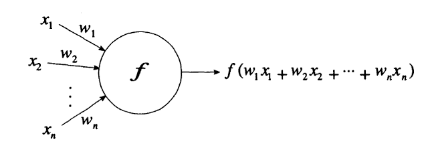
\includegraphics{NeuronExample.PNG}
		\caption{An example of a basic neuron in a neural network. Input 
		$x_1...x_n$ together with a weight $w_1...w_n$ are put into function 
		$f$ to create output. \cite{rojas2013neural}}
		\label{fig:NeurEx}
	\end{figure}

	\begin{figure}[h!]
		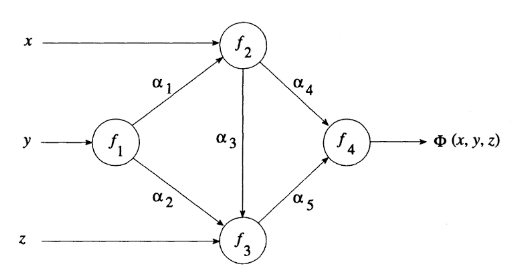
\includegraphics{NeuralNetworkExample.PNG}
		\caption{An example of a neural network consisting of neurons (Figure 
		\ref{fig:NeurEx}). \cite{rojas2013neural}}
		\label{fig:NeurNetEx}
	\end{figure}
	
	% Neural Networks layers
	These created networks are divided in layers. The first layer is the 
	collection of all neurons that have an external input value. The last layer 
	is the collection of all neurons that generate output values. All layers in 
	between are called hidden layers, as a user cannot see those neurons from 
	the outside.\cite{Wang2003}
	
	% Training neural networks
	As explained in the section about machine learning, the neural network must 
	be trained (Section \ref{subsec:MachineLearning}). This can be done after 
	the architecture is defined. Again, with the data, a training and a test 
	set must be made, as well. With those, the neural network can be properly 
	trained to create the right output when giving values as an input. 
	\cite{Wang2003}
	
	\subsubsection{Convolutional Neural Networks}
	
	% Introduction Convolutional Networks
	A more specific variant of neural networks is a convolutional neural 
	network (CNN). CNNs combine neural networks and convolutions to reduce 
	noise in the signal and approximate the actual input better. Convolutions 
	use kernels to use the values close to the input it wants to approximate. 
	It also uses pooling, which makes the input smaller by approximating a 
	location and its nearby inputs into one. \cite{Goodfellow-et-al-2016}
	
	\clearpage
	
	\subsection{Deep Learning Frameworks}
	
	% Introduction Deep Learning frameworks
	A wide selection of deep learning frameworks are available. Most of these 
	frameworks are implemented in Python, with some exceptions. A selection of 
	the five most popular are explained, together with their advantages and 
	disadvantages.
	
	\subsubsection{Skikit-learn Python}
	
	% Introduction Skikit-learn
	Python itself has a package that can be used for machine learning, named 
	Skikit-learn. It is high-level interactive and is maturing in a quick rate, 
	due to its usage in both the academic world as in the industry. It also has 
	some C++ libraries incorporated, but makes most use of the three packages 
	Numpy, Scipy and Cython. Due to his high-level and ease of use, a drawback 
	is its computational efficiency and therefore is not the best choice for 
	testing large data sets.\cite{pedregosa2011scikit}
	
	\subsubsection{Theano}
	
	% Introduction Theano
	Theano is one of the open source machine learning frameworks written in 
	Python.\cite{bergstra2010theano} Its programming is declarative. 
	\cite{rampasek2016tensorflow} This one uses the famous NumPy syntax for 
	higher computation speed 
	in its language. It was developed mainly to simplify the implementation of 
	the the algorithms used for well performing machine learning. Two tasks 
	that are intensive for the processor, either training a multi-layer neural 
	or a convolutional network. Theano works through a pipeline on compilation 
	(Figure \ref{fig:TheanoPipe}). At first it puts the graph in standard form 
	(Canonicalization). Next it improves the stability of the computation 
	(stabilization). Thirdly it replaces expressions with faster ones 
	(Specialization). Fourth it moves the computation to the GPU, if compiled 
	for GPU (GPU transfer). In the last step it loads Python modules with 
	specialized implementations (Code Generation). \cite{bergstra2010theano}
	
	\begin{figure}[h!]
		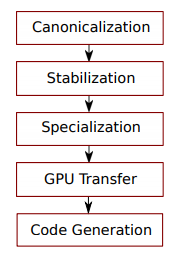
\includegraphics{TheanoPipeline.PNG}
		\caption{The steps Theano takes in compilation for functions for GPU. 
		\cite{bergstra2010theano}}
		\label{fig:TheanoPipe}
	\end{figure}
	
	% Theano extensions
	Theano has been seen as a base for many other neural network creation 
	frameworks. Examples are Keras, Lasagne, GroundHog, Blocks and Pylearn2. It 
	utilizes from the benefits of being written in Python, such as creating a 
	friendly enviroment for fast and easy interaction with data. However, since 
	threading is done by Python, it is not possible to have multiple 
	interpreters going on at the same time. The graph optimization time, code 
	compilation and memory usage time all can be improved. \cite{al2016theano}
	
	\subsubsection{TensorFlow}
	
	% Introduction TensorFlow
	TensorFlow, also open sourced, is developed for experimentation on new 
	models, training those models with the help of large datasets and at last 
	move those models into production.\cite{abadi2016tensorflow} Tensorflow 
	is 
	declarative and made in C++, while also having interfaces in Python. 
	\cite{rampasek2016tensorflow} Google makes regular use of TensorFlow, 
	as an example. However many more programmers use TensorFlow for their 
	applications. It is a follow-up of the earlier system DistBelief and 
	simplified and generalized that. TensorFlow is mainly supporting training 
	and inference on a larger scale. It uses a dataflow graph for representing 
	the computation within the algorithm and the operation state of the 
	algorithm. \cite{abadi2016tensorflow}
	
	% Phases TensorFlow
	While executing a TensorFlow application, two different phases can be 
	distinguished. The first phase of the two makes a to be trained neural 
	network and the update rules in the form of a dataflow graph. The places 
	for input are reserved by place holders for state representation. The 
	second phase is the earlier neural network after optimization. Because of 
	these two phases, the execution phase can be optimized with the information 
	of the computation. There will not be any intermediate results slowing down 
	the process. \cite{abadi2016tensorflow}
	
	Not only Theano, but TensorFlow as well has some wrappers, too. Keras (also 
	for Theano) and Pretty Tensor both use TensorFlow as a base for creating 
	neural networks. \cite{rampasek2016tensorflow}
	
	\subsubsection{Caffe}
	
	% Introuction Caffe
	Caffe is a framework based on the C++ library together with Python and 
	MATLAB. Caffe, too, is open sourced and its programming is imperative. 
	\cite{rampasek2016tensorflow} It is very useful for researches as 
	its code is modular and its network definitions are well separated. The 
	test coverage of Caffe is useful as well, as every new module has a test 
	and is not accepted without a test. The bindings with python and MATLAB 
	makes constructing networks and classifying inputs easier. At last does 
	Caffe provide pre-trained reference models. This makes it easier to 
	reproduce research.
	\cite{DBLP:journals/corr/JiaSDKLGGD14}
	
	\subsubsection{Torch}
	
	% Introduction Torch
	Torch is an object-oriented framework for machine learning and is 
	implemented in Lua, but also has interfaces in C. Torch is also 
	imperative.\cite{rampasek2016tensorflow} A modular strategy was used to 
	simplify any 
	modifications of existing algorithms. There are four classes chosen. The 
	first class is about data handling (DataSet). The second one is the black 
	box that gives an output (Machine). The third is the class that is used to 
	find the optimal set of parameters (Trainer). The last one is about 
	printing the measures of interest (Measurer). These classes give a very 
	clear general idea. Several examples of usable machines are the gradient 
	machines, support vector machines and distributions. 
	\cite{collobert2002torch}
	
	\subsubsection{Comparing Frameworks}

	% Kovalev comparisons
	Kovalev compared the likings of Theano (with Keras extension), Torch, 
	Caffe, TensorFlow and the not discussed Deeplearning4J based on convergence 
	and prediction time, classification accuracy and framework complexity 
	(lines of code). Both the depth (number of internal layers) and the width 
	(number of neurons within fixed number of layers). When regarding training, 
	prediction and testing times, all but DeepLearning4J were performing quite 
	well. When watching Classification accuracy, Torch and Tensorflow performed 
	visibly instable and Caffe seemed to be a bit worse overall. The last 
	comparison, framework complexity was best for Theano, followed by 
	TensorFlow and then Caffe. From best to worst the article rated the 
	following order: Theano (with Keras), TensorFlow, Caffe, Torch, 
	Deeplearning4J.	\cite{kovalev2016deep}

	% Caffe comparisons
	The creator of Caffe compared its own framework with other known 
	frameworks. The focus was mainly on basic parts of the programs, namely BSD 
	licence, core and binding languages CPU and GPU coverage, Open source, 
	training and the availability of pretrained models. Caffe has the advantage 
	in comparison with the earlier described Theano and Torch regarding binding 
	languages and the availability of pretrained 
	models.\cite{DBLP:journals/corr/JiaSDKLGGD14}
	
	\begin{figure}[h!]
		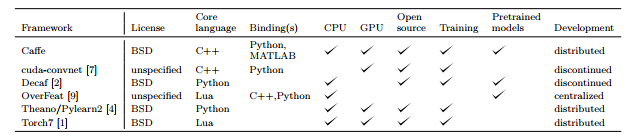
\includegraphics{CaffeMachineLearningComparisons.PNG}
		\caption{The comparisons between different machine learning frameworks 
		from Caffe creator point of view. 
		\cite{DBLP:journals/corr/JiaSDKLGGD14}}
		\label{fig:CaffeMachLearnComp}
	\end{figure}

	% Bahrampour's comparisons
	Bahrampour tested Caffe, Theano, Torch and the not discussed Neon on their 
	extensibility, hardware utilisation and speed for both CPU and GPU usage. 
	He stated that Caffe, Theano and Torch were at that moment the top three 
	well developed and used frameworks. Neon was added because of its 
	potential. The speed was measured by a forward time (check time it takes 
	for a pre-selected batch) and a gradient computation time (time for each 
	measurable parameter). The conclusion of the research had six parts: Theano 
	and then Torch are the most extensible. For both CPU- and GPU-based 
	training and deployment Theano and Torch are fighting for the number one 
	spot. Torch would benefit from expansion in both documentation and 
	debugging, though. \cite{bahrampour2016comparative}

	% Chi's comparisons
	Another research that compared deep learning framework was Shi. The 
	frameworks Caffe, TensorFlow and Torch were tested by him, as well as the 
	not discussed CNTK from Microsoft and MXNet. The tests that were done about 
	speed were on CPUs, one GPU and multiple GPUs on both synthetic and real 
	data. The overal outcome was that Caffe, CNTK and MXNet performed better 
	than TensorFlow and Torch, although TensorFlow's production ramped up with 
	more threads.
	\cite{DBLP:journals/corr/ShiWXC16}


	% Fox's comparisons
	Similar to Bahrampour\cite{bahrampour2016comparative}, Fox compared 
	TensorFlow, Caffe, Theano, Torch and the not discussed CNTK, 
	Deeplearning4j, MXNet and H2O, for them being open-source, relatively 
	mature and adopted by the community. He mainly discussed the different 
	frameworks and afterwards made a table with all those findings (Figure 
	\ref{fig:FramewComps}). \cite{fox2016software}
	
	\begin{figure}[h!]
		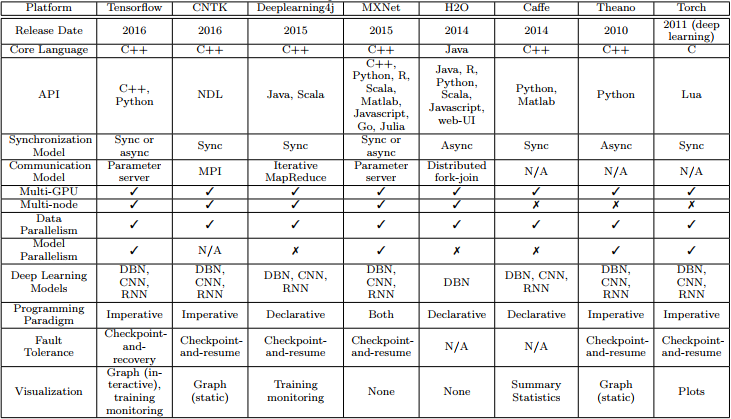
\includegraphics[scale=0.8]{FrameworkComparisons.PNG}
		\caption{Comparisons of eight frameworks. The comparisons were 
		implementation based.}
		\label{fig:FramewComps}
	\end{figure}
	
	% Parvat's comparisons
	Parvat had a more listings approach in comparing the frameworks Theano, 
	Caffe, Torch, Tensorflow and the not discussed Deeplearning4J and NVIDIA 
	cuDNN. This time they were compared on their platform, interface, modelling 
	capability, support for CUDA, OpenMP, OpenCL and support for pre-trained 
	models. He concluded that TensorFlow was very flexible, due to being more 
	than a deep learning framework. Theano is very helpful for creating models 
	fast, especially with the libraries, and therefore TensorFlow and Theano 
	are the most flexible. Torch is good because of the pre-trained models, 
	however misses being written in a mainstream language. Caffe is useful when 
	working with images, and also has a lot of pre-trained CNN models. 
	Deeplearning4j has its advantage being the only one working with Java and 
	Scala. 
	At last TensorFlow has the advantage of being able to work with a 
	distributed environment. \cite{parvat2017survey}
	
	 A last article to discuss about comparing deep learning frameworks is 
	 written by Erickson. Erickson focused on language, environment, speed and 
	 maturity. Caffe, being the most mature one and very fast, has a 
	 disadvantage when tuning hyperparameters. TensorFlow is regarded as hard 
	 to use directly, however has good performance and tools for help. Theano 
	 is similar as TensorFlow, in that it has good performance, however is a 
	 bit harder to learn. Both of these frameworks can be made more user 
	 friendly with a library as Keras. Keras uses the performance of either 
	 TensorFlow or Theano and can be used easily to create models with 
	 efficient code. Also Torch is given a good maturity level and good 
	 documentation. \cite{erickson2017toolkits}
	
	% Final conclusions
	As can be seen by the many articles written about these frameworks, there 
	is not a clear distribution as to which framework should be used when. It 
	seems that Theano and TensorFlow, especially with help from libraries such 
	as Keras are regarded a bit better than the others. On the other hand Caffe 
	has some advantages, too.
	
	\bibliography{../References/Citings} 
	\bibliographystyle{ieeetr}
	
\end{document}
